\documentclass[final,leqno]{siamltex}

\usepackage{amsmath,amssymb,amsfonts,algorithm,algorithmic,multirow,booktabs,graphicx}
\DeclareMathOperator{\prox}{prox}

\title{OUR REPORT TITLE\thanks{This report was conducted as part of the Columbia ECBM E6040 final project.}} 

\author{Zichen Chao\footnotemark[2] \and Shenlong Gu\footnotemark[2] \and Kan Zhu\footnotemark[2] \and Yibo Zhu\footnotemark[3]}

\begin{document}
\maketitle

\renewcommand{\thefootnote}{\fnsymbol{footnote}}

\footnotetext[2]{Department of Computer Science, Columbia University in the City of New York.}
\footnotetext[3]{Department of Industrial Engineering and Operations Research, Columbia University in the City of New York.}

\slugger{siopt}{xxxx}{xx}{x}{x--x}
\begin{abstract} 
In this paper, we realize the result of the paper ReNet: A Recurrent Neural Network Based Alternative to Convolutional Networks \cite{renet} using Python's Deeplearning Library $\textit{Theano}$.

\end{abstract} 

\begin{keywords}
Recurrent Neural Networks, Convolutional Neural Networks, Theano
\end{keywords}

\pagestyle{myheadings}
\thispagestyle{plain}

\section{Introduction}
\subsection{Motivation}
Convolution Neural Networks(CNN) have proven its power in object recognition and image classification problems. Previous works of Recurrent Neural Networks(RNN) also shows great performance in handwriting recognition/generation and speech recognition. Rather than the multi-dimensional RNN inspired before, one could use a uni-dimensional RNN, which makes each output activation of the layer be computed with respect to the whole input image, rather than the local extracted activation computed in CNN. Also, comparing to multi-dimensional RNN, the number of RNNs at each layer scales could bes linear with respect to the number of dimensions $d$ of the input image ($2d$), while multi-dimensional RNN requires the exponential number of RNNs at each layer ($2^d$). Furthermore, parallelizability could be easier, as each RNN is dependent only along a horizontal or vertical sequence of patches. 
\subsection{Related Work}
The idea of using RNN on offline handwriting recognition is from Graves and Schmidhuber's paper\cite{multidimrnn}. They use Multi-dimensional RNN (MDRNN), which avoids any alphabet specific preprocessing and thus could be applicable for any language, with the help of connectionist temporal classification algorithm. The challenging part of offline problem comparing to online problem is that the input is no longer one dimensional, hence if the image shifts vertically by one pixel, it would be completely different. 
Other related works aiming at classification of images is summarized in a github website \cite{imgcls}. 

\subsection{Organization}

The rest of the paper is organized as follows. We review the model architecture of ReNet in \S \ref{background}. Then we recreate the result of ReNet in \S \ref{result}. Lastly, \S \ref{discussion} concludes the paper and gives direction for future work.

\section{Background} \label{background} 
The ReNet paper proposed a deep neural network architecture for object recognition based on recurrent neural networks(RNN). The proposed network, called ReNet, replaces the ubiquitous convolution+pooling layer of the deep convolutional neural network with four recurrent neural networks that sweep horizontally and vertically in both directions across the image. \\

First, we sweep the image vertically with two RNNs, with one RNN working in a bottom-up direction and the other working in a topdown direction. Each RNN takes as an input one (flattened) patch at a time and updates its hidden state, working along each column $j$ of the split input image $X$.\\

After this vertical, bidirectional sweep, we concatenate the intermediate hidden states (forward and backward) at each location of patch to get a composite feature map. Each state is now the activation of a feature detector at the corresponding location with respect to all the patches in the $j$-th column of the original input. Next we sweep over the obtained feature map horizontally with two RNN. In a similar manner as the vertical sweep, these RNNs work along each row resulting in the output feature map. Now, each vector represents the features of the original image patch in the context of the whole image.\\

The functions are as follows:
\begin{eqnarray}
	v_{i,j}^F = f_{VFWD}(z_{i,j-1}^F, p_{i,j}) \text{~for } j=1,\dots,J \nonumber \\
	v_{i,j}^R = f_{VREV}(z_{i,j+1}^R, p_{i,j}) \text{~for } j=J,\dots,1 \nonumber
\end{eqnarray}

The schema are as follows:\\
\begin{center}
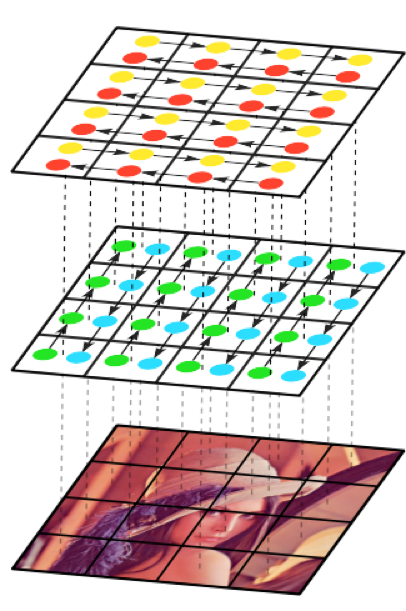
\includegraphics[scale=0.45]{Figures/Picture1}
\end{center}

They evaluate the proposed ReNet on three widely-used benchmark datasets; MNIST, CIFAR-10 and SVHN. The result suggests that ReNet is a viable alternative to the deep convolutional neural network, and that further investigation is needed.


\section{Result} \label{result}

\section{Discussion} \label{discussion}
\subsection{Future Work}
First, we evaluated the proposed ReNet only quantitatively. However, the accuracies on the test sets do not reveal what kind of image structures the ReNet has captured in order to perform object recognition. Further investigation along the line of regularization of neural networks using dropconnect is necessary, as well as exploring ensembles which combine RNNs and CNNs for bagged prediction.\\

Second, we can use many parallelization tricks which are widely used for training CNN such as parallelizing fully-connected layers, having separate sets of kernels/features in different processors and exploiting data parallelism.\\

Third, this mechanism can be applied to multidimensional grid other than image. We can applied the algorithm to 3D real object detection.
\section*{Contribution}

\bibliographystyle{siam.bst}
\bibliography{bibl}

\end{document}